\section{Static analysis}\label{sec-static}

In this section we discuss a real-life application that benefits from static
analysis of effectful computations -- the \Dune build system~\citep{dune}. We
start by introducing \Dune and motivating the need for static analysis with
over-approximation (\S\ref{sec-dune-intro}), and then show how one can implement
static analysis of build system dependencies using selective functors
(\S\ref{sec-static-example}).

\subsection{Dune build system}\label{sec-dune-intro}

\Dune was originally developed at Jane Street and has by now become a standard
build system for OCaml packages~\citep{dune}. At the time of writing, more than
1000 OCaml packages are using \Dune as the build system. The original motivation
for developing \Dune (earlier known as \cmd{jbuilder}) was to make it easier
to open source code developed in an industrial environment, and so \Dune was not
meant to be used for everyday software development. However, \Dune's ability to
extract maximum parallelism from build scripts meant it was faster than existing
build systems, such as \textsc{OCamlbuild}, and it quickly became popular, with
major projects switching to \Dune, for example, the \textsc{Coq} proof
assistant~\citep{bertot2013coq}.

% TODO: Can we get any performance improvement figures on how much more
% parallelism can be gained through static analysis?

One unusual feature of \Dune is the ability to statically
over-approximate all build dependencies of a package. This is used at
Jane Street to automatically produce \emph{package manifest files} for
more than 100 packages instead of maintaining them by hand. Package
manifest files are consumed by \emph{package managers}, such as
OPAM~\citep{opam}, which download and install all required dependencies
\emph{before the build starts}.

% The original aim of this feature was to automatically generate package manifest
% files, so that they do not need to be maintained. An alternative approach would
% be to integrate the build system with the package manager itself, i.e. whenever
% the build system discovers a new external dependency, the package manager would
% download and install it, temporarily suspending the build.

% The reason Dune could not follow this approach is because package managers are
% typically designed to be build system agnostic.

% There are also optional package dependencies. Shall we give more details?

To generate a manifest file automatically \Dune needs to analyse the build graph
statically, i.e. \emph{without actually running any build commands}, because at
this point the project cannot yet be built (due to missing dependencies).
Package dependencies can be conditional and depend on values that can only be
computed during the build, therefore in many situations it is impossible to
statically compute an exact set of dependencies, and hence an over-approximation
is used instead.

In general, one can view such static dependency analysis as a function from a
build script to a set of package dependencies, and implement it directly by
parsing the script and extracting all possible dependencies from it. \Dune
adopts a different approach: it reuses the existing script execution engine that
executes build commands, but in a mock environment where commands are skipped,
but their dependencies are recorded in all branches of conditional statements.
By doing static analysis at this level, one can reuse a lot of code, e.g. for
parsing and interpreting build scripts.

In this mock environment, some parts of the code cannot be fully evaluated as
they need the output produced by external commands. However, these parts still
need to be analysed. To achieve this, the original implementation of \Dune uses
the \emph{arrow} abstraction discussed in~\S\ref{sec-arrows}. To evaluate
suitability of selective functors for this task, we have successfully prototyped
an alternative core for \Dune, which uses applicative and selective functors
instead of arrows.

% The reason Dune uses an arrow
% rather than an applicative is discussed later, however applicatives
% would be suitable as well in this context. In particular, a
% successful attempt was made at replacing arrows by applicatives in
% Dune in the past.

\subsection{Static analysis of build dependencies}\label{sec-static-example}

\Dune is written in OCaml, and we therefore developed an OCaml library for
selective functors. In this section, however, we choose to continue using
Haskell to avoid confusion.

We follow the approach by~\citet{mokhov2018build} for modelling \emph{build
tasks}, where a single task is represented as a higher-order effectful function
parameterised by the type of \emph{keys} \hs{k}, e.g. file names, and the type
of \emph{values} \hs{v}, e.g. file contents. A task takes a \emph{callback} of
type \hs{k}~\hs{->}~\hs{f}~\hs{v}, that the task can use to find values of its
dependencies, and returns the result embedded in a selective context~\hs{f}:

\vspace{1mm}
\begin{minted}[xleftmargin=10pt]{haskell}
newtype Task k v = Task { run :: forall f. Selective f => (k -> f v) -> f v }
\end{minted}
\vspace{1mm}

\noindent
The task needs to be polymorphic over the \hs{f} so that it can be run both in
\emph{build mode}, by actually executing build commands, and in the \emph{mock
mode}, where build commands are skipped but dependencies are recorded, as
explained in \S\ref{sec-dune-intro}. For example, to compute over- and
under-approximation of build dependencies we can run the task in selective
functors \hs{f}~\hs{=}~\hs{Over} and \hs{f}~\hs{=}~\hs{Under}, respectively:

\vspace{1mm}
\begin{minted}[xleftmargin=10pt]{haskell}
dependenciesOver :: Task k v -> [k]
dependenciesOver task = getOver $ run task (\k -> Over [k])

dependenciesUnder :: Task k v -> [k]
dependenciesUnder task = getUnder $ run task (\k -> Under [k])
\end{minted}
\vspace{1mm}

\noindent
Thanks to the polymorphism of \hs{Task} over \hs{f}, we can ``execute'' a given
task with a mock callback like
\hs{(\}\hs{k}~\hs{->}~\hs{Over}~\hs{[}\hs{k])}~\hs{::}~\hs{k}~\hs{->}~\hs{Over}~\hs{[}\hs{k]}~\hs{v},
whose only effect is recording the given key.

To demonstrate this on an example, we need a way to model a \emph{build script},
i.e. a collection of build tasks. One simple approach~\citep{mokhov2018build}
is to use a function that, given a key~\hs{k} returns either the corresponding
build \hs{Task} or \hs{Nothing} to indicate that this key is an input~(external)
dependency that cannot be built and should therefore be available before the
build starts:

\vspace{1mm}
\begin{minted}[xleftmargin=10pt]{haskell}
type Script k v = k -> Maybe (Task k v)
\end{minted}
\vspace{1mm}

\noindent
Now we have all the ingredients for creating a simple build script comprising
two tasks: (i)~the top-level task for building \cmd{release.tar} by archiving
the file \cmd{LICENSE} and the executable \cmd{exe}; and (ii)~the task for
compiling the executable from the source \cmd{src.ml} and one of the two
libraries: \cmd{lib.c} or \cmd{lib.ml}, depending on the configuration option
stored in the \cmd{config} file (it is common to use an optimised low-level C
implementation of a performance-critical function, falling back to high-level
OCaml implementation if the former is unavailable on the system):

\vspace{1mm}
\begin{minted}[xleftmargin=10pt]{haskell}
script :: Script FilePath String
script "release.tar" = Just $ Task $ \fetch -> tar [fetch@\,@"LICENSE",@\,\blk{fetch}\,@"exe"]
script "exe" = Just $ Task $ \fetch ->
    let src   = fetch "src.ml"
        cfg   = fetch "config"
        libc  = fetch "lib.c"
        libml = fetch "lib.ml"
    in compile [src, ifS (parse cfg) libc libml]
script _ = Nothing
\end{minted}
\vspace{1mm}

\noindent
We assume the existence of functions \hs{tar} (creating an archive),
\hs{compile} (compiling an OCaml executable from sources and libraries), and
\hs{parse} (parsing a configuration file); their implementation is irrelevant
for our purposes.

\begin{figure}
\centerline{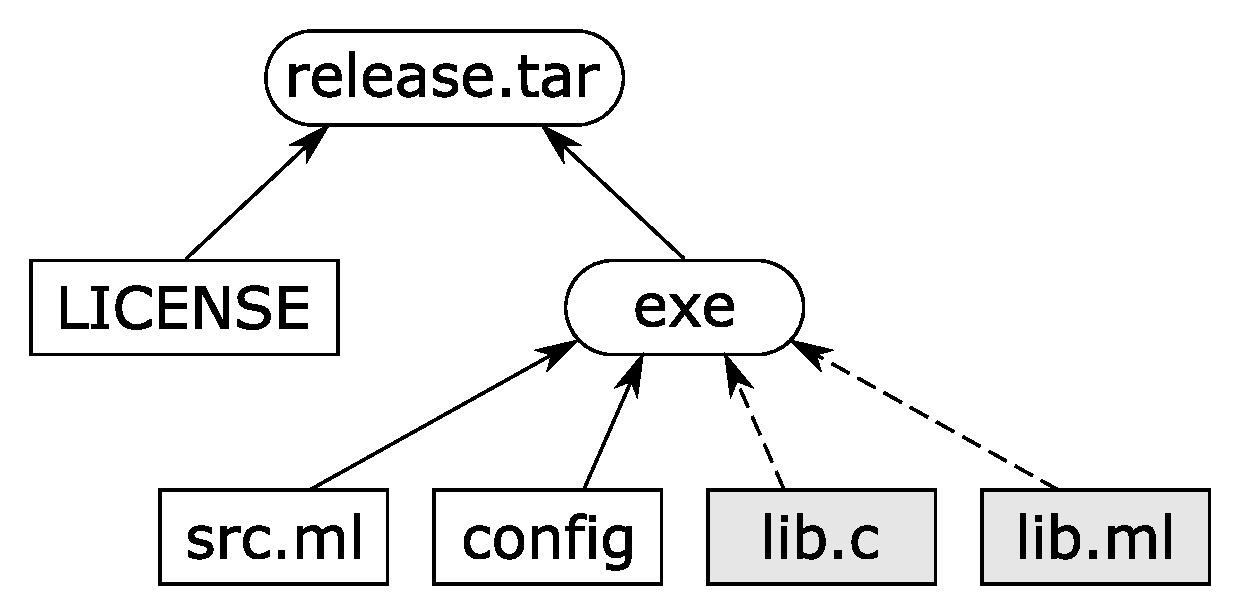
\includegraphics[scale=0.3]{fig/build-dependencies.pdf}}
\caption{An example build dependency graph. Input files are shown in rectangles,
intermediate and output files are shown in rounded rectangles. Approximate
dependencies are highlighted with dashed lines.}
\label{fig-build}
\end{figure}

By analysing individual build tasks using \hs{dependenciesOver} and
\hs{dependenciesUnder}, we can obtain an approximate build dependency
information for the whole dependency graph:

\vspace{1mm}
\begin{minted}[xleftmargin=10pt]{haskell}
@\ghci@ dependenciesOver (fromJust $ script "release.tar")
["LICENSE","exe"]
@\ghci@ dependenciesUnder (fromJust $ script "release.tar")
["LICENSE","exe"]
@\ghci@ dependenciesOver (fromJust $ script "exe")
["src.ml","config","lib.c","lib.ml"]
@\ghci@ dependenciesUnder (fromJust $ script "exe")
["src.ml","config"]
\end{minted}
\vspace{1mm}

\noindent
Fig.~\ref{fig-build} visualises the graph obtained by traversing approximate
dependencies starting from the target key \cmd{release.tar}.

Note that while over-approximation is useful for installing all possible
dependencies \emph{before the build}, under-approximation is useful for
maximising parallelism \emph{during the build}: for example, if all input files
in our example are actually generated, e.g. by running a text preprocessor, then
we can start the three preprocessing tasks that are definitely needed
(\cmd{LICENSE}, \cmd{src.ml}, \cmd{config}) in parallel, i.e. without waiting
for the outcome of parsing the \cmd{config} file.

\emph{Applicative and monadic build systems} studied in~\citep{mokhov2018build}
cannot support such over- and under-approximating static analysis, and the
associated abstractions are therefore unsuitable for \Dune. This explains why
\Dune developers have chosen to use the \emph{arrow} abstraction
(\S\ref{sec-arrows}). As our case study and the developed prototype demonstrate,
selective functors provide a viable alternative to arrows in the context of
build systems.

% Dune is another example where the extra power provided by selective
% functions is relevant. To understand why, let's consider the following
% example: a user wants to use some optimized C function if it is
% available on the system, and fallback to an OCaml implementation if
% not. The C and OCaml implementations might have different external
% dependencies. Such a test is dynamic since it depends on the system
% the users builds the software on. During compilation, we only want to
% follow one of the branch, as we clearly don't want to build
% implementation only to keep a single one. However, during dependency
% analysis for the project manifest we need to scan both branches. The
% dependencies discovered in both branches will be considered as
% optional dependencies given that neither is always required.

% For parallelism use underapproximation: take intersection of optional
% dependencies, and then union with necessary dependencies.
% Note that this requires 'branch' to be in the type class, so we
% can see both branches and intersect their effects.
